\documentclass{beamer}
\usepackage{pgf,tikz}
\usetikzlibrary{arrows}
 \usetheme{Warsaw}
\usepackage{amsmath, amssymb, mathrsfs, amsopn, amsfonts, amstext,color}
\usepackage{graphicx}
\beamertemplatenavigationsymbolsempty

\definecolor{cnuBlue}{RGB}{0,44,118}
\definecolor{cnuAthletic}{RGB}{0,57,116}
\definecolor{cnuGray}{RGB}{165,172,176}
\definecolor{cnuSilver}{RGB}{132,136,139}
\definecolor{red}{RGB}{255,0,0}

\title[Stallman Biography]{Richard Stallman Biography}
\date{}
\subtitle{Mathematical Writing 301}
\author[Hayhurst]{John Wesley McDonald Hayhurst}

\begin{document}

\section{Richard Stallman Biography}
\subsection{Stallman Biography}
\begin{frame}\frametitle{Introduction}
\maketitle
\end{frame}

\begin{frame}\frametitle{Richard Stallman}
  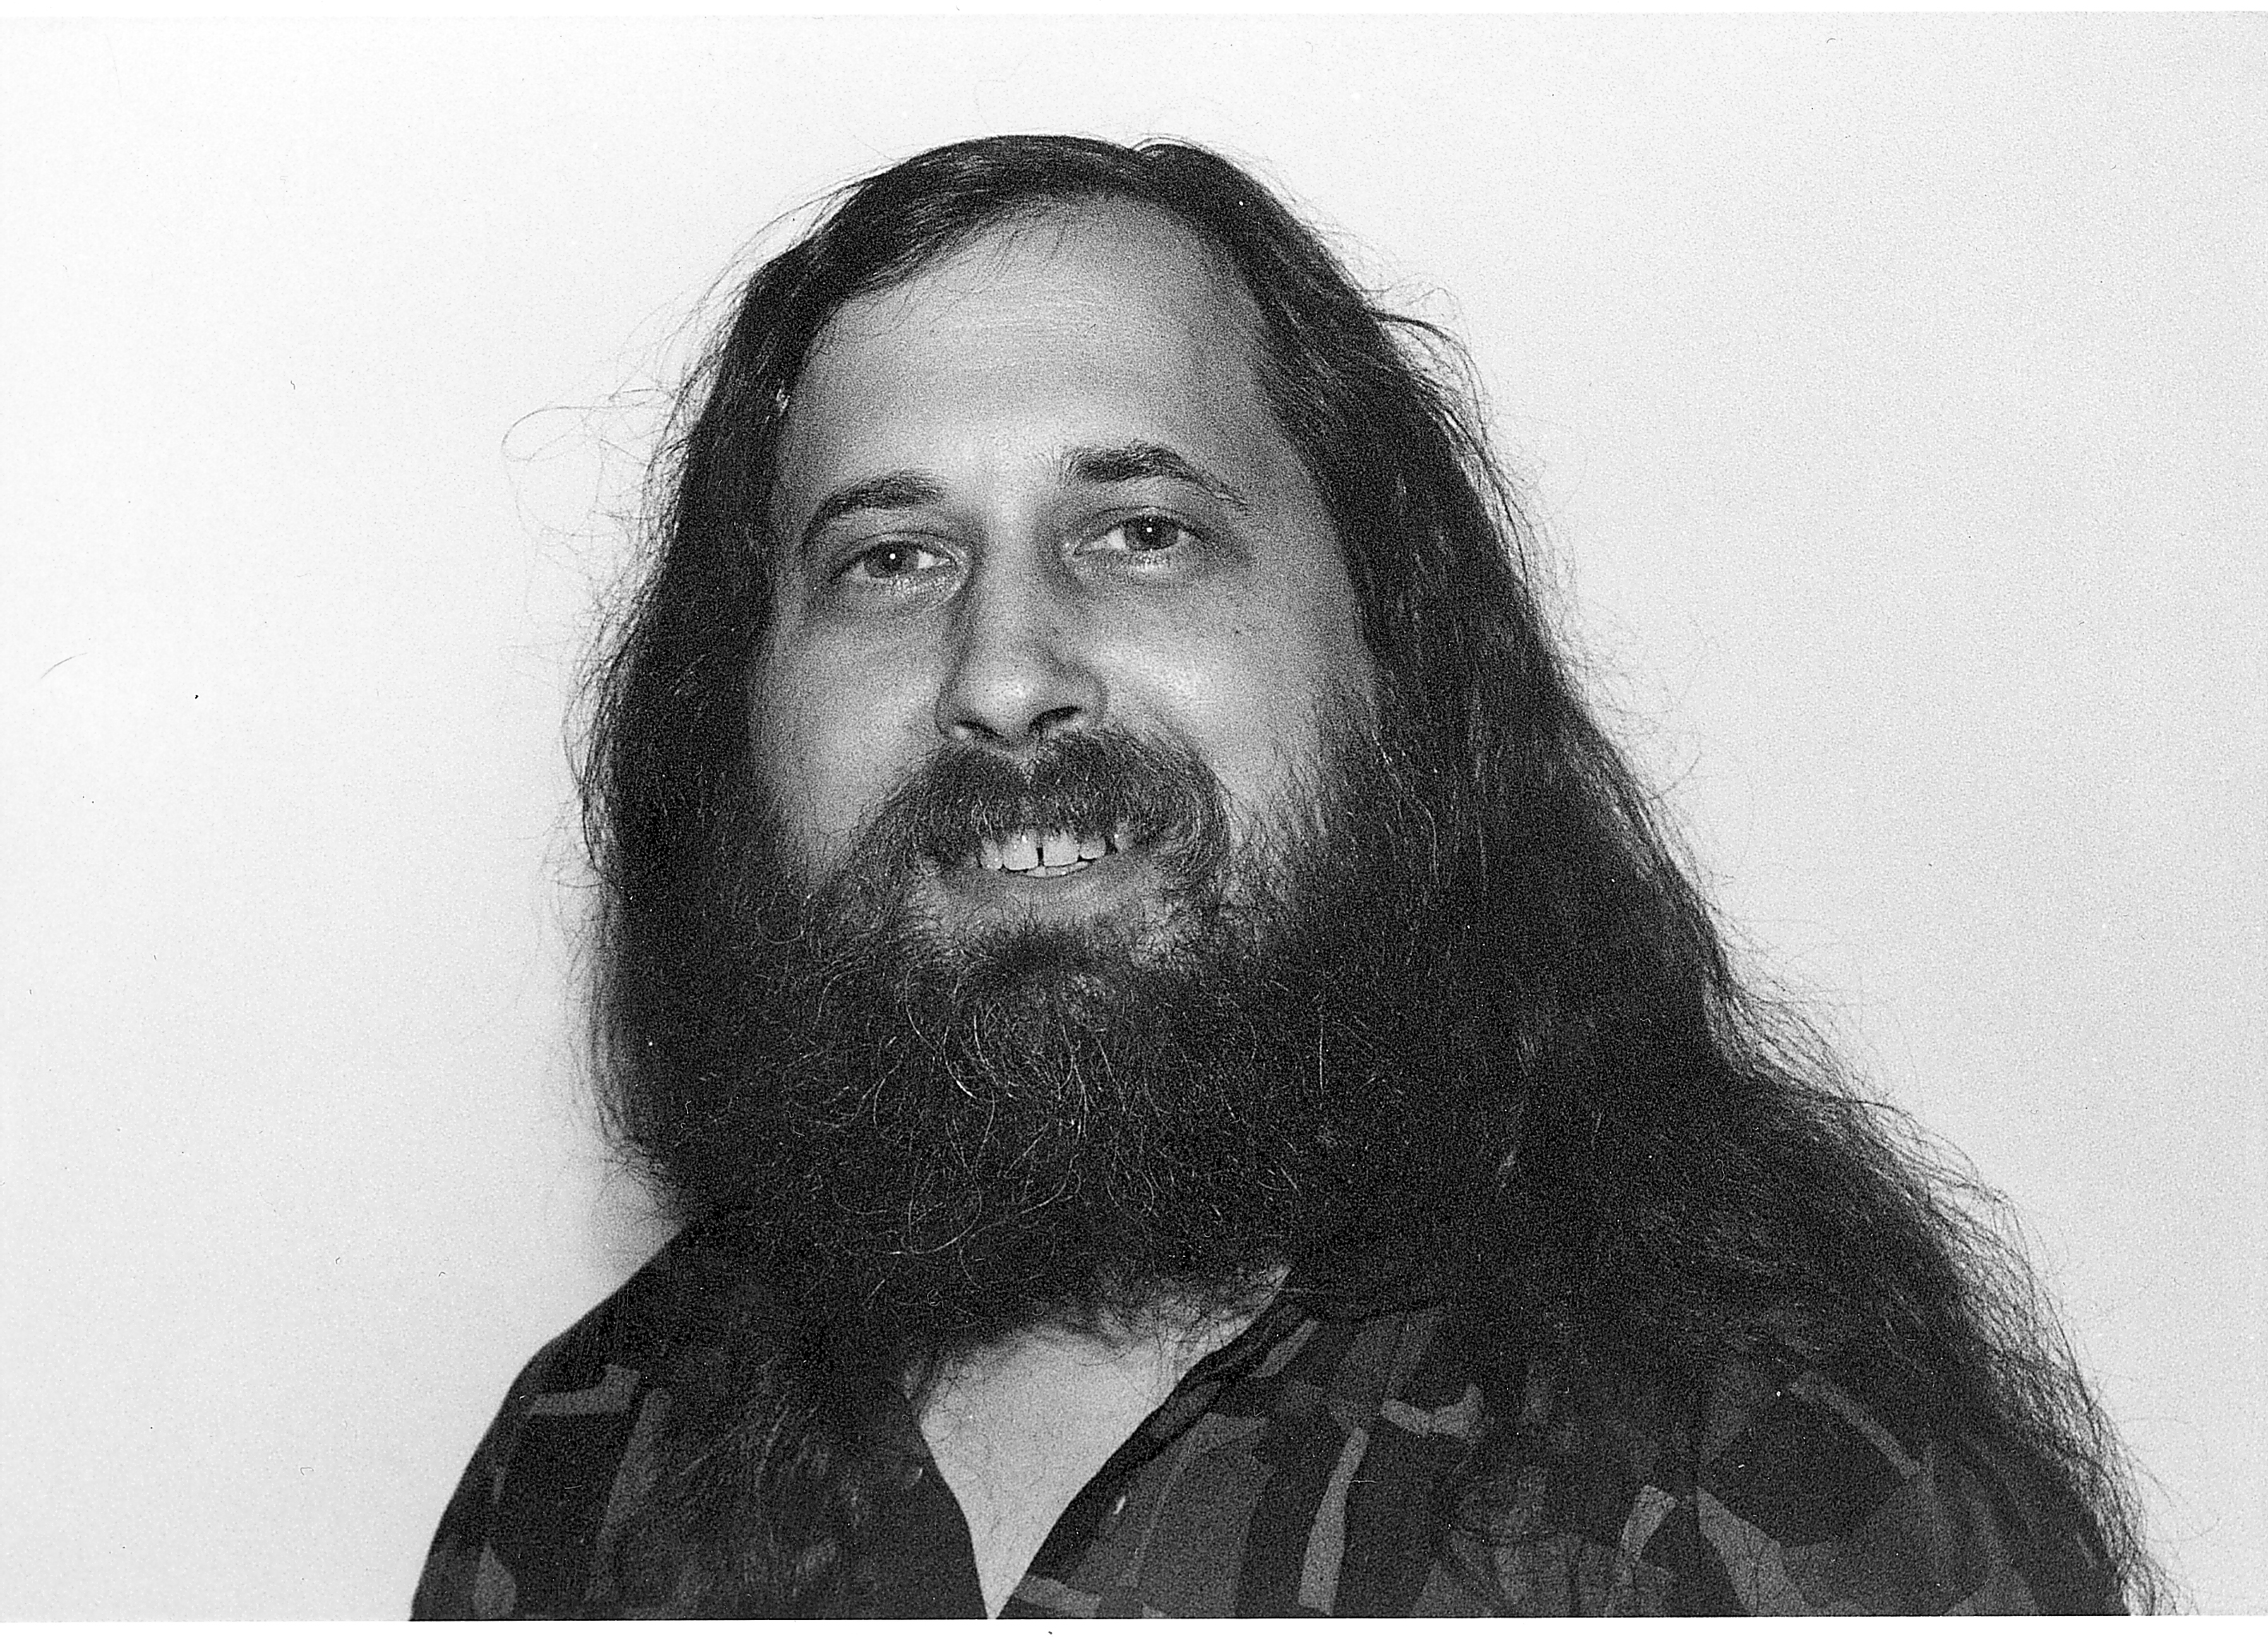
\includegraphics[scale=.6, center]{stallman1.jpg} \\
  \begin{center}
    \small{Pictured: Richard Stallman (1)}
  \end{center}
\end{frame}


\begin{frame}\frametitle{Early Life}
  \begin{itemize}
    \item Stallman was born to Alice Lippman and Daniel Stallman in New York 1953.
    \item He showed an early interest in computers and attended Columbia University Saturday program, IBM New York Scientific Center.
    \item He attended Harvard in which his first year he became a programmer at MIT Artificial Intelligence Laboratory.
    \item He graduated from Harvard magna cum laude in physics in 1974.
    \item He attended MIT for graduate research and while there published a paper with Garry Sussman detailing dependency-directed backtracking. Which is still used to this day.
  \end{itemize}
\end{frame}

\begin{frame}\frametitle{Stallman}
  \begin{center}
    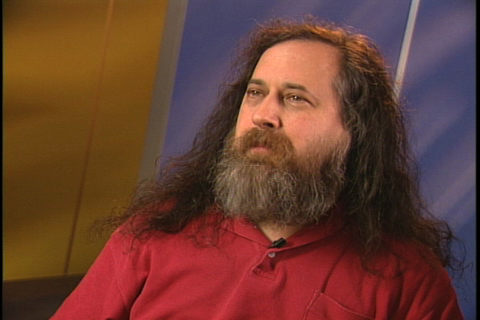
\includegraphics[scale=.5, center]{stallman2.jpg}\\
    \small {Pictured: Richard Stallman (2)}
  \end{center}

\end{frame}

\begin{frame}\frametitle{GNU}
  \begin{itemize}
    \item Later in his career Stallman got frustrated with the current state of computer software.
    \item He disliked the privatization of code and believed that software should be free.
    \begin{itemize}
      \item This is the idea of free as in freedom, not free as in beer.
    \end{itemize}
    \item Following this philosophy, he announced the GNU Operating System in 1983.
    \item He created some of the necessary tools including a text editor (emacs), compiler (GCC), and a build automator (GNU make).
    \item Additionally he created the GNU General Public License (GPL) which was a legal document protecting taking code and selling it.
  \end{itemize}
\end{frame}

\begin{frame}\frametitle{GNU}
  \begin{itemize}
    \item Unfortunately by 1990, Stallman had not created a kernel for the proposed GNU operating system.
    \item Fortunately, Linus Torvalds had created a kernel using the existing projects Stallman had created.
    \item With a kernel (created by Linus) and basic programs to use, the operating system called GNU/Linux was released.
  \end{itemize}
\end{frame}

\begin{frame}\frametitle{Linus Torvalds}
  \begin{center}
    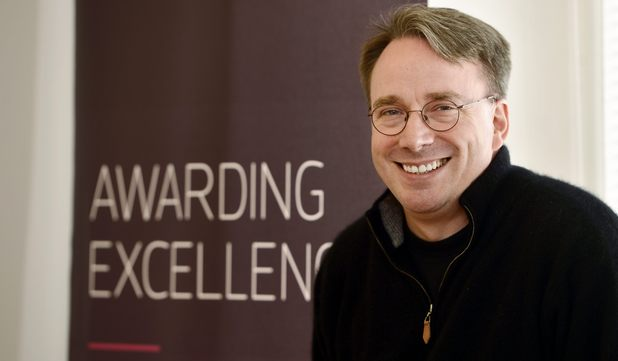
\includegraphics[scale=1.6, center]{linus1.jpg}\\
    \small{Pictured: Linus Torvalds}
  \end{center}
\end{frame}

\begin{frame}\frametitle{Activism}
  \begin{itemize}
    \item While Stallman has a lifetime of computer work under his belt, he is most known for his activism
    \item He has promoted world wide the notion of free software
    \begin{itemize}
      \item He has met with Hugo Ch{\'a}vez
      \item was on the Advisory Council for the TV station teleSUR.
    \end{itemize}
    \item He has criticized ATI, Apple, and Steve Jobs for the privatization of software.
    \item He also actively fights against copyright law suggesting that copyright should only be 10 years long.
    \item He helped the International Music Score Library Project come back online after it was taken down.
  \end{itemize}
\end{frame}

\begin{frame}\frametitle{Accomplishments and Awards}
  \begin{itemize}
    \item He has won over 23 awards in his life
    \item Grace Murray Hopper Award "For pioneering work in the development of the extensible editor EMACS"
    \item Holds over 12 Honorary Doctorates
    \item Holds over 4 Honorary Professorships
    \item Exceptional merit award from the MacArthur Fellowship
  \end{itemize}
\end{frame}

\begin{frame}\frametitle{Personal Life}
  \begin{itemize}
    \item Richard Stallman's personal life is, "interesting", to say the least.
    \item He does not celebrate Christmas but rather celebrates Grav-mass which celebrates Isaac Newton instead.
    \item He supports the National Initiative, The Green Party, Paper voting, not using Skype,and not owning a cell phone.
    \item If you were wondering, he supports Bernie Sanders for the 2016 Presidential Election.
  \end{itemize}
\end{frame}

\begin{frame}\frametitle{Bibliography}
  \begin{itemize}
    \item Contributors - Using the GNU Compiler Collection (GCC). \textit{Contributors - Using the GNU Compiler Collection (GCC)}. http://gcc.gnu.org/onlinedocs/gcc/Contributors.html
    \item Make Your Open Source Software GPL-Compatible. Or Else. \textit{Make Your Open Source Software GPL-Compatible. Or Else}. http://www.dwheeler.com/essays/gpl-compatible.html
    \item Staff and Board. \textit{Free Software Foundation Working Together for Free Software}. http://www.fsf.org/about/staff-and-board
    \item Chavez TV beams into South America. \textit{The Guardian}. Guardian News and Media. http://www.theguardian.com/media/2005/jul/26/venezuela.broadcasting
    \item Richard Stallman's Personal Page. \textit{Richard Stallman's Personal Page}. https://stallman.org/
  \end{itemize}
\end{frame}

\begin{frame}\frametitle{Bibliography}
  \begin{itemize}
    \item Richard Stallman (1). Digital image. https://stallman.org/image001.jpg.
    \item Richard Stallman (2). Digital image. http://archive09.linux.com/var/uploads/Image/articles/147983-1.jpg.
    \item Linus Torvalds. Digital image. http://i1-news.softpedia-static.com/images/news2/linus-torvalds-says-people-who-believe-in-an-ai-singularity-are-on-drugs-486373-2.jpg
  \end{itemize}
\end{frame}
\end{document}
